\documentclass{article}
\usepackage{graphicx}
\usepackage{url}
\usepackage{natbib}

\begin{document}
\title{Supplement to \\``Rapid, accurate peptide identification''}

\author{Chris Y. Park, Aaron A. Klammer, Lukas K\"{a}ll, \\
Michael J. MacCoss and William S. Noble}

\maketitle

\begin{figure}
  \centering
  \begin{tabular}{ll}
    {\sf A} & {\sf B} \\
    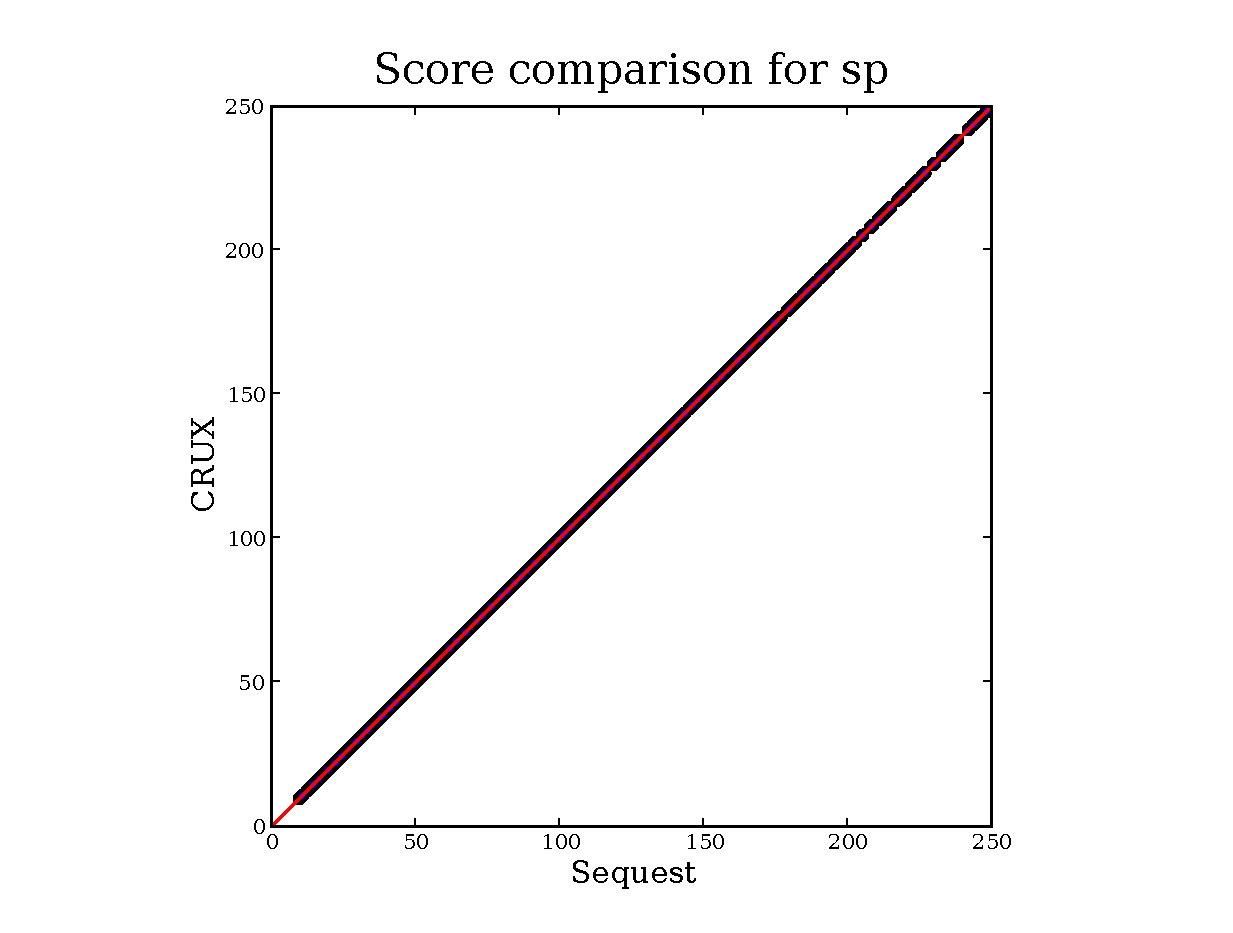
\includegraphics[width=2.5in]{../../results/paper-figure/second-score/4800/fig-2-random-sp.eps} &
    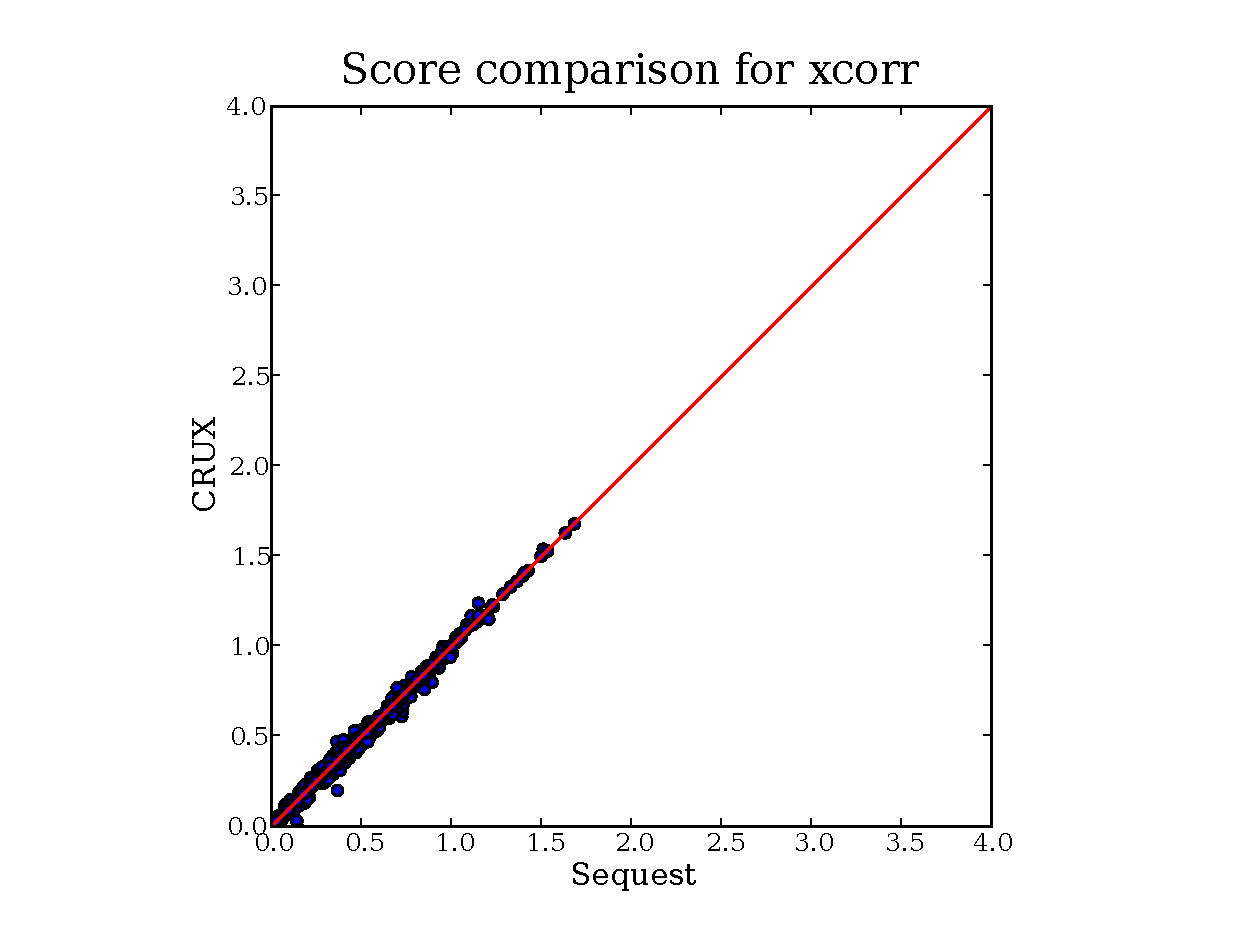
\includegraphics[width=2.5in]{../../results/paper-figure/second-score/4800/fig-2-random-xcorr.eps} \\
    {\sf C} & {\sf D} \\
    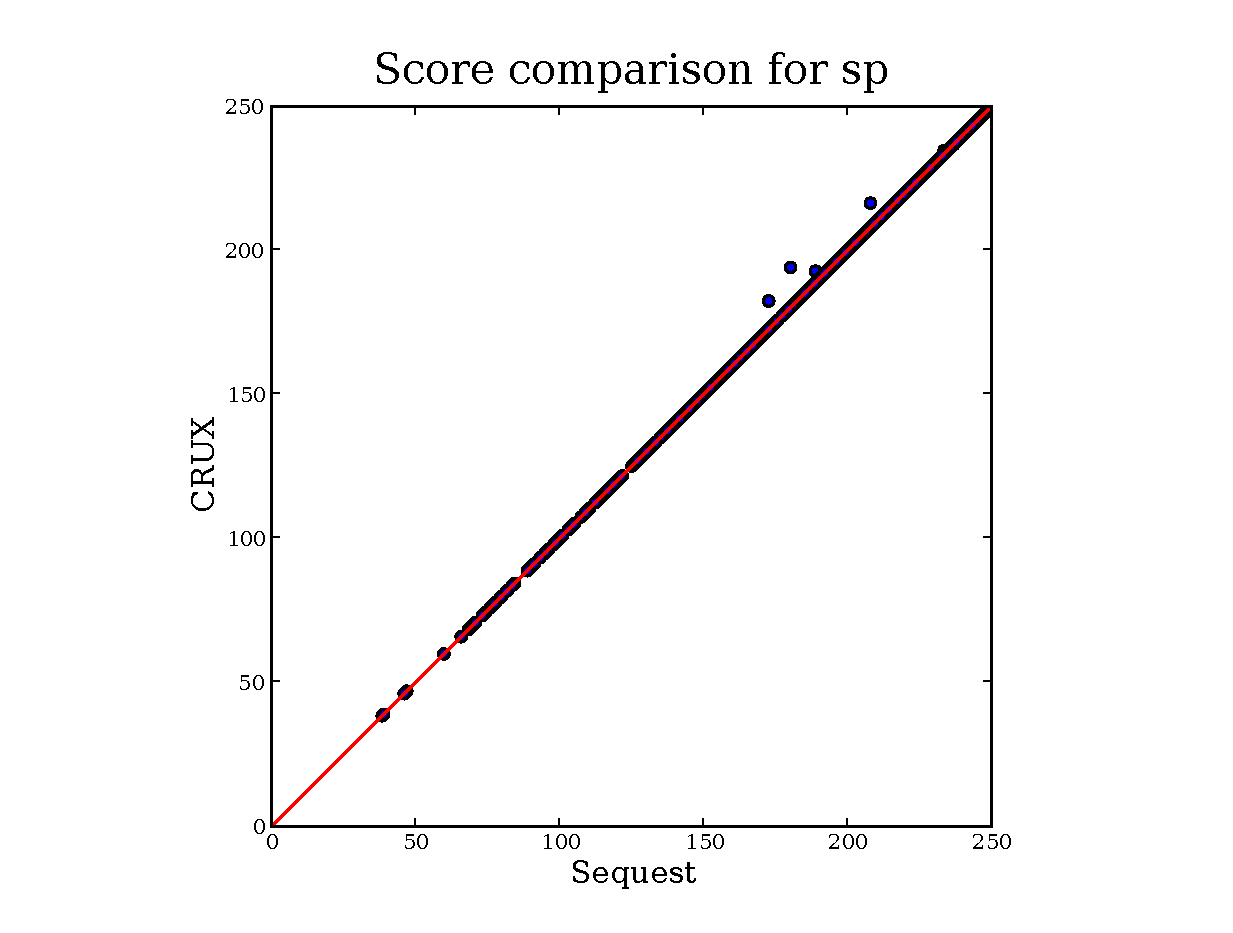
\includegraphics[width=2.5in]{../../results/paper-figure/second-score/QSTAR/fig-2-random-sp.eps} &
    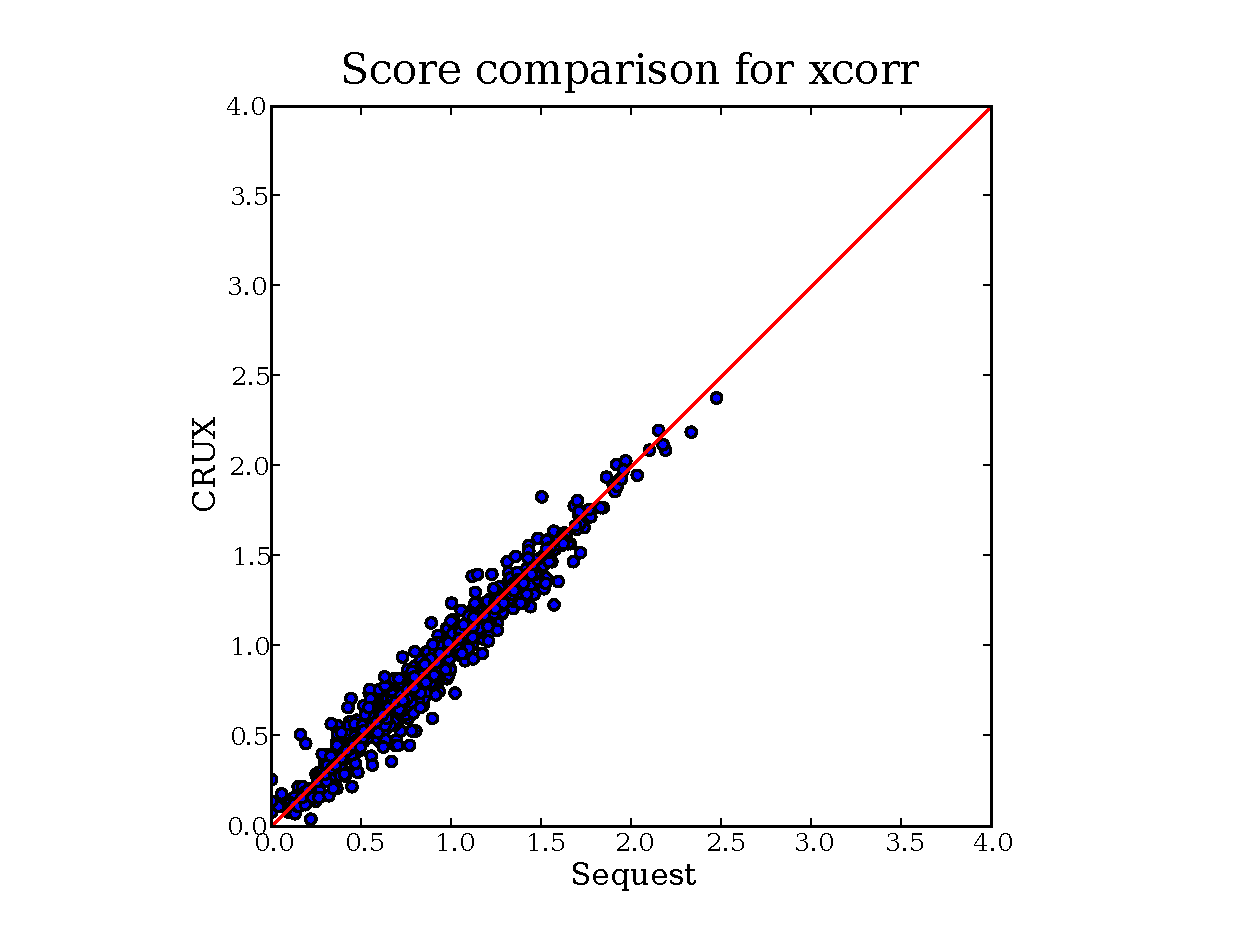
\includegraphics[width=2.5in]{../../results/paper-figure/second-score/QSTAR/fig-2-random-xcorr.eps} \\

  \end{tabular}
  \caption{{\bf Re-implementation of $Sp$ and $Xcorr$ scoring functions.}
  The figure plots, for a collection of MALDI-TOF/TOF spectra (top, {\sf A}
  and {\sf B}) and QTOF spectra (bottom, {\sc C} and {\sc D}) scored against 
  randomly associated peptides using $Sp$ (left, {\sf A} and {\sf C}) and 
  $XCorr$ (right, {\sf B} and {\sf D}) 
  as computed by Crux as a function of the
  same scores as computed by {\sc Sequest}. The spectra obtained 
  are 1000 spectra randomly sampled from the 4800 and QStar data sets
  publicly available at 
  http://pubs.acs.org/cgi-bin/abstract.cgi/jprobs/2008/7/i01/abs/pr070244j.html
 \citep{klimek:standard}.
  \label{figure:sp-xcorr-random}}
\end{figure}

\begin{figure}
  \centering
  \begin{tabular}{ll}
    {\sf A} & {\sf B} \\
  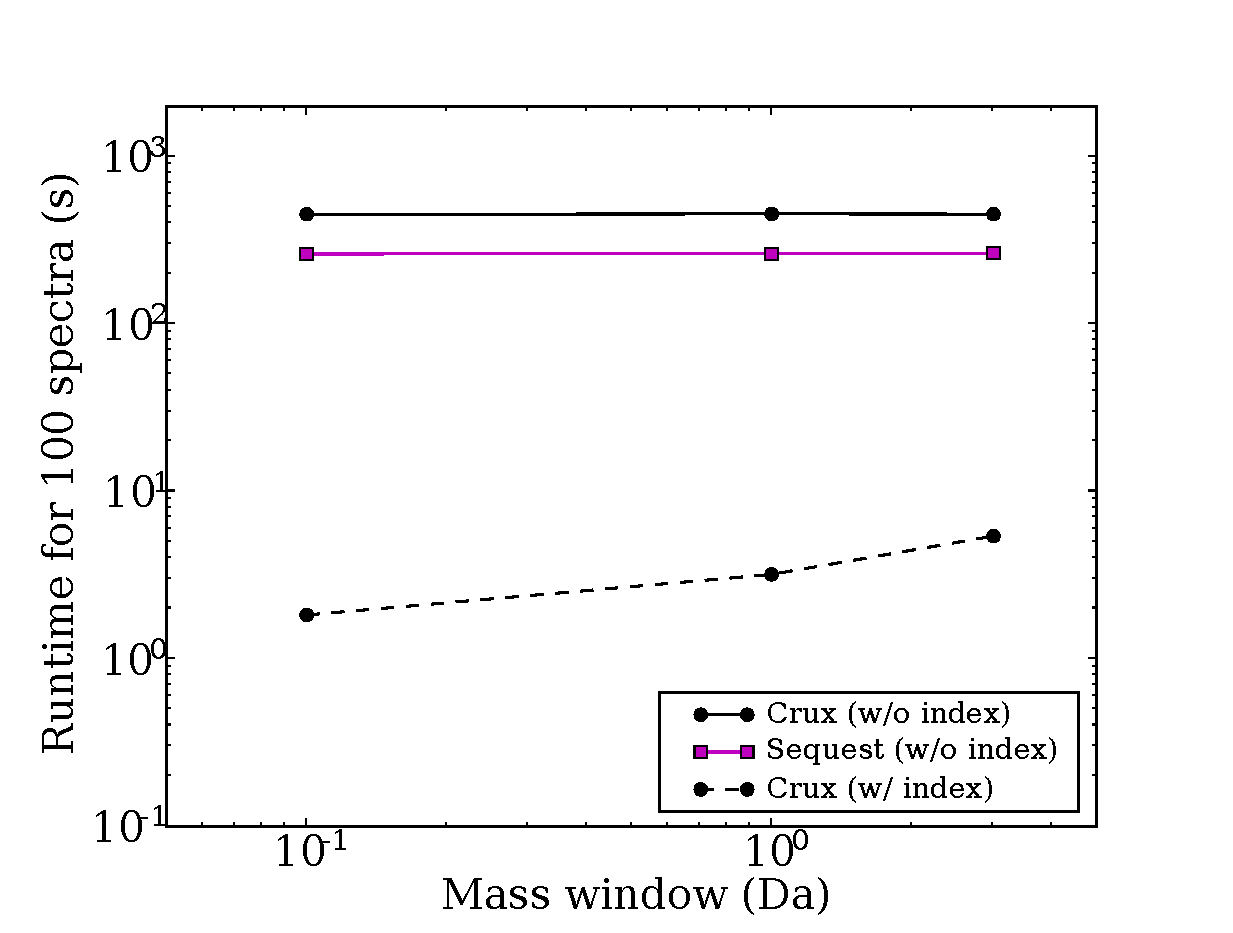
\includegraphics[width=2.5in]{../../results/paper-figure/index/indexing-yeast.eps} &
  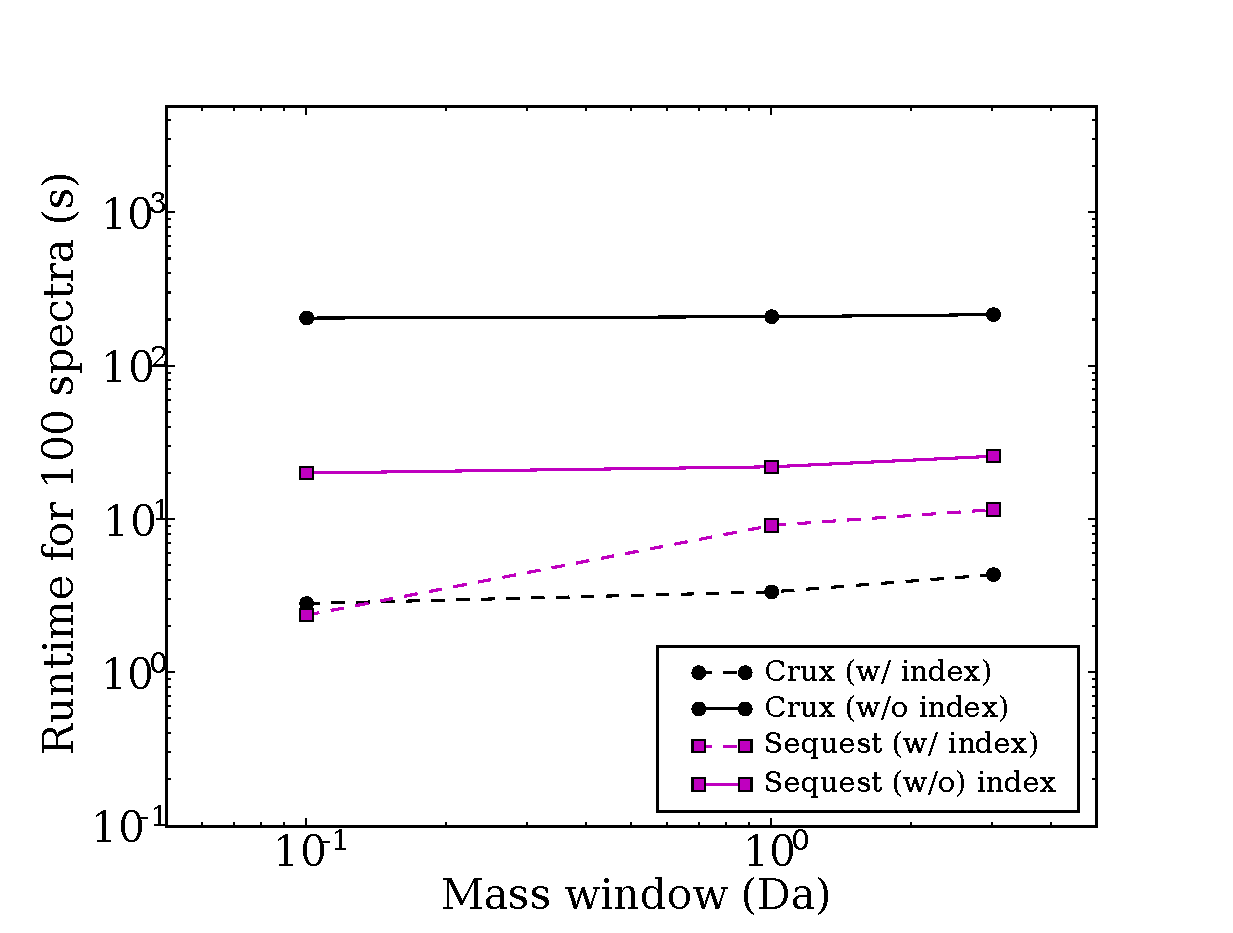
\includegraphics[width=2.5in]{../../results/paper-figure/turbo-no-missed/indexing-yeast-windows.eps} \\

\end{tabular}
  \caption{{\bf Rapid retrieval of candidate peptides.}  The figure
  plots the total running time required to search 100 tandem mass
  spectra against the yeast protein databases
  on computers running the Linux ({\sf A}) 
  or Windows ({\sf B}) operating systems, using {\sc Sequest} and Crux with 
  and without indices.
  Run time is plotted 
  as a function of the mass tolerance used to define candidate
  peptides. The Linux OS plots have three series
  because indexed {\sc Sequest} searches with are only possible on Windows.
  \label{figure:indexing}}
\end{figure}

\bibliographystyle{plos}
\bibliography{refs}

\end{document}
